\section{Лекция 7}
\subsection{XIV. Нестационарная теория возмущений (квантовая теория переходов).}
\subsection{\S XIV.1 Переходы под действием слабого возмущения.}
Гамильтониан квантовой системы
\[
\hat{H}^{(S)}(t) = \hat{H}_0^{(S)} + \hat{V}^{(S)}(t),
\]
где невозмущенный гамильтониан $H_0$ не зависит от времени. Является ли $H$ интегралом движения?
\[
\dfrac{d\hat{H}^{(S)}}{dt} = \dfrac{\partial\hat{H}^{(S)}(t)}{\partial t} + \dfrac{i}{\hbar}\left[\hat{H}^{(S)}(t),~\hat{H}^{(S)}\right] = \dfrac{\partial(\hat{H}_0^{(S)} + \hat{V}^{(S)}(t))}{\partial t} = \dfrac{\partial\hat{V}^{(S)}(t)}{\partial t} = 0
\]
$\Longrightarrow$ не существует стационарных уровней $E_n$, но есть уровни $E_n^{(0)}$ невозмущенного гамильтониана $\hat{H}_0^{(S)}\ket{E_n^{(0)}} = E_n^{(0)}\ket{E_n^{(0)}}$.\\

Основной вопрос нестационарной теории: в момент времени $t_0$ было состояние $E_i^{(0)}$, какова вероятность $w\left(t_1,~ E_f^{(0)}~|~t_0,~E_i^{(0)}\right)$?





\subsection{\S XIV.1.1 Возмущение, действующее в течение конечного промежутка времени.}
Перейдем в представлении взаимодействия, предполагая, что $t_0 = 0$:
\[
\hat{H}_0^{(S)} = \hat{H}^{(I)} =: \hat{H}_0,\tab \ket{\psi^{(I)}(t)} = e^{\dfrac{i}{\hbar}\hat{H}_0t}\ket{\psi^{(S)}(t)}, \tab \ket{\psi^{(I)}(t = 0)} = \ket{\psi^{(S)}(t = 0)} = \ket{\psi_i^{(0)}}.
\]

Выразим через $S$-матрицу:
\[
\ket{\psi^{(I)}(t)} = \hat{S}(t,~0)\ket{\psi_i^{(0)}},
\]
где $\hat{S}(t,~0) = \hat{T}\left(e^{\dfrac{i}{\hbar} \int\limits_0^t d\tau \hat{V}^{(I)}(\tau)}\right)$.\\

Теория возмущений применима, если возмущение мало. Как это влияет на наше выражение? Можем разложить экспоненту в ряд Тейлора, тогда, пренебрегая слагаемыми после первого, получим
\[
\hat{S(t,~0)} = \hat{1} - \dfrac{i}{\hbar}\int\limits_0^td\tau\hat{V}^{(I)}(\tau)
\]
Здесь мы избавились от $\hat{T}$, т.к. упорядочивать нечего. Тогда, подставляя в выражение для вектора состояния:
\[
\ket{\psi^{(I)}(t)} = \ket{\psi_i^{(0)}} - \dfrac{i}{\hbar}\int\limits_0^td\tau\hat{V}^{(I)}(\tau)\ket{\psi_i^{(0)}} = \ket{\psi_i^{(0)}} + \ket{\delta\psi^{(1)}(t)}
\]
Рассмотрим финальное состояние $\ket{\psi_f^{(0)}}$: $\hat{H_0}\ket{\psi_f^{(0)}} = E_f^{(0)}\ket{\psi_f^{(0)}}$, $\braket{\psi_i^{(0)}}{\psi_f^{(0)}} = 0$. Найдем вероятность $W_{if}(t) = \left|\braket{\psi_f^{(0)}}{\psi^{(I)}(t)}\right|^2= \left|\braupket{\psi_f^{(0)}}{\hat{S}(t,~0)}{\psi_i^{(0)}}\right|^2$.
\[
\braupket{\psi_f^{(0)}}{\hat{S}(t,~0)}{\psi_i^{(0)}} \approx -\dfrac{i}{\hbar}\int\limits_0^td\tau\braupket{\psi_f^{(0)}}{\hat{V}^{(I)}(\tau)}{\psi_i^{(0)}} = -\dfrac{i}{\hbar}\int\limits_0^td\tau\braupket{\psi_f^{(0)}}{e^{\dfrac{i}{\hbar}\hat{H_0}t}\hat{V}^{(S)}(\tau)e^{-\dfrac{i}{\hbar}\hat{H_0}t}}{\psi_i^{(0)}} = (*)
\]
Т.к. $\psi_i$ и $\psi_f$ --- собственные функции $H_0$
\[
(*) = -\dfrac{i}{\hbar}\int\limits_0^t d\tau~e^{\dfrac{i}{\hbar}\left(E_f^{(0)} - E_i^{(0)}\right)t}\braupket{\psi_f^{(0)}}{\hat{V}^{(S)}(\tau)}{\psi_i^{(0)}} = (*)
\]
Введем частоту перехода из $\psi_i$ в $\psi_f$ $\omega_{fi} = \dfrac{i}{\hbar}\left(E_f^{(0)} - E_i^{(0)}\right)$ и $V_{fi}(\tau) = \braupket{\psi_f^{(0)}}{\hat{V}^{(S)}(\tau)}{\psi_i^{(0)}}$, тогда
\[
(*) = -\dfrac{i}{\hbar}\int\limits_0^td\tau~ e^{i\omega_{fi}\tau}V_{fi}(\tau)
\]
Тогда, считая, что этот интеграл существует,
\[
W_{if} = \dfrac{1}{\hbar^2}\left|\int\limits_0^td\tau~ e^{i\omega_{fi}\tau}V_{fi}(\tau)\right|^2
\]


Рассмотрим интересный нам частный случай.
\begin{figure}[H]
	\centering
	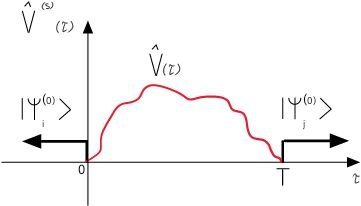
\includegraphics[width=0.75\linewidth]{images/s15_1(1).jpeg}
\end{figure}
Здесь
\[
\hat{V}^{(S)}(\tau) = \begin{cases}
	0,\ \text{если }\tau<0\text{ или } \tau > T\\
	\hat{V}(\tau), \ \text{если }\tau\in[0,~T]
\end{cases}
\]
При $\tau < 0$ система находилась в состоянии $\ket{\psi_i^{(0)}}$, которое является собственной функцией $H_0$. Какова вероятность того, что при $\tau > T$ система перейдет в состояние $\ket{\psi_f^{(0)}}$?
\[
W_{fi} = \dfrac{1}{\hbar^2}\left|\int\limits_0^Td\tau~ e^{i\omega_{fi}\tau}V_{fi}(\tau)\right|^2 = \dfrac{1}{\hbar^2}\left|\int\limits_{-\infty}^{+\infty}d\tau~ e^{i\omega_{fi}\tau}V_{fi}(\tau)\right|^2
\]
Вспомним преоьразование Фурье: $V_{fi} = \int\limits_{-\infty}^{+\infty} \dfrac{d\tau}{\sqrt{2\pi}}e^{i\omega\tau}V_{fi}(\tau)$, с учетом чего
\[
W_{fi} = \dfrac{2\pi}{\hbar^2}\left|V_{fi}(\omega)\right|^2
\]

Если взять в качестве возмущения $\hat{V}^{(S)}(t) = \hat{F}e^{-i\omega t} + \hat{F}^\dagger e^{i\omega t}$, то при $\omega \neq \dfrac{1}{\hbar}\left| E_f^{(0)} - E_i^{(0)}\right|$ переходов не будет.\\

Рассмотрим еще один важный частный случай.
\begin{figure}[H]
	\centering
	\includegraphics[width=0.75\linewidth]{images/s15_2(1).jpeg}
\end{figure}
В момент $t_1$ система находилась в состоянии $\ket{\psi_i^{(0)}}$, которое является собственной функцией $H_0$. Какова вероятность того, что в момент $t_2$ система будет в состоянии $\ket{\psi_f^{(0)}}$?\\

Обозначим $\braupket{\psi_f^{(0)}}{\hat{V}_0}{\psi_i^{(0)}} = \tilde{V}_{fi}$, это почти константа, тогда:
\[
W_fi(\Delta t = t_2 - t_1) = \dfrac{|\tilde{V}_{fi}|^2}{\hbar^2}\left|\int\limits_{t_1}^{t_2}d\tau~e^{i\omega_{fi}\tau}\right|^2 = \dfrac{4|\tilde{V}_{fi}|^2}{(\hbar\omega_{fi})^2}\sin{^2(\omega_{fi}\Delta t)}
\]
Но при $\hat{V}\approx const$ должна работать стационарная теория возмущений, а там нет переходов между уровнями. Как тогда правильно учесть "хвост" графика?
\[
\braupket{\psi_f^{(0)}}{\hat{S}(T, 0)}{\psi_i^{(0)}} = -\frac{i}{\hbar} \int\limits_0^T d\tau e^{i\omega_{fi}\tau} V_{fi}(\tau) = \dfrac{i}{\hbar}\left[\int\limits_0^td\tau~\dfrac{d}{d\tau}\left(\dfrac{e^{i\omega_{fi}\tau}V_{fi}(\tau)}{i\omega_{fi}}\right) - \int\limits_0^td\tau~\dfrac{e^{i\omega_{fi}\tau}}{i\omega_{fi}}\dfrac{d V_{fi}(\tau)}{d\tau}\right] = (*)
\]
С учетом того, что $V_{fi}(0) = 0$, $V_{fi}(t) = \tilde{V_{fi}}$, получим
\[
(*) = \dfrac{i}{\hbar}\left[-\dfrac{e^{i\omega_{fi}t}\tilde{V}_{fi}}{i\omega_{fi}} + \int\limits_0^td\tau~\dfrac{e^{i\omega_{fi}\tau}}{i\omega_{fi}}\dfrac{d V_{fi}(\tau)}{d\tau}\right]
\]
При первом порядке стационарной теории было бы
\[
\ket{\psi_f^{(0)}} \longrightarrow \ket{\psi_f} = \ket{\psi_f^{(0)}} + \dfrac{\tilde{V_{fi}}}{E_f^{(0)} - E_i^{(0)}}\ket{\psi_i^{(0)}} = \ket{\psi_f^{(0)}} + \dfrac{\tilde{V_{fi}}}{\hbar\omega_{fi}}\ket{\psi_i^{(0)}}
\]
Значит на самом деле ищем переход не в $\ket{\psi_f^{(0)}}$, а в состояние, которое было "поправлено" после смещения спектра $\Longrightarrow$ за вероятность в получившемся выше выражении отвечает второе слагаемое.
\[
W_{fi}(t) = \dfrac{1}{(\hbar\omega_{fi})^2}\left|\int\limits_0^td\tau~e^{i\omega_{fi}\tau}\dfrac{d V_{fi}(\tau)}{d\tau}\right|^2,
\]
что сходится теперь и сос тационарным случаем.



\subsection{\S XIV.1.2 Внезапное и адиабатическое включение возмущение (в рамках \textit{теории возмущений}).}
\begin{definition}
	Возмущение меняется \textbf{адиабатически}, если $\left|\dfrac{d V_{fi}(t)}{dt}\right| << |V_{fi}(t)|\cdot \omega_{fi}$.
\end{definition}
\begin{definition}
	Возмущение называется \textbf{внезапным}, если $\left|\dfrac{d V_{fi}(t)}{dt}\right|\Bigg|_{t=0} \longrightarrow + \infty$, т.е. возмущение "включается" в момент $t = 0$.
\end{definition}

Пусть \(\hat{V}^{(S)}(t)\) действует на участке \([0, T]\), причем \(\hat{V}^{(S)}(t=0) = \hat{V}^{(S)}(t=T) = 0\). Тогда

\[
\braupket{\psi_f^{(0)}}{\hat{S}(T, 0)}{\psi_i^{(0)}} = -\frac{i}{\hbar} \int\limits_0^T d\tau e^{i\omega_{fi}\tau} V_{fi}(\tau).
\]


Интегрируя по частям, получим

\[
\braupket{\psi_f^{(0)}}{\hat{S}(T, 0)}{\psi_i^{(0)}} = -\frac{e^{i\omega_{fi}\tau} V_{fi}(\tau)}{\hbar \omega_{fi}} \Bigg|_0^T + \frac{1}{\hbar \omega_{fi}} \int\limits_0^T d\tau e^{i\omega_{fi}\tau} \frac{dV_{fi}(\tau)}{d\tau}.
\]

\[
\Longrightarrow \braupket{\psi_f^{(0)}}{\hat{S}(T, 0)}{\psi_i^{(0)}} = \frac{1}{\hbar \omega_{fi}} \int\limits_0^T d\tau e^{i\omega_{fi}\tau} \frac{dV_{fi}(\tau)}{d\tau}.
\]
\begin{enumerate}
	\item \textit{Адиабатическое возмущение.}\\
	В интеграле можем считать, что \(\dfrac{dV_{fi}(\tau)}{d\tau} = const\),
	$\braupket{\psi_f^{(0)}}{\hat{S}(T, 0)}{\psi_i^{(0)}} \approx \left|\dfrac{d V_{fi}(\tau)}{d\tau}\right|\Bigg|_{t=\tilde{t}}\dfrac{1}{\hbar \omega_{fi}} \int\limits_0^Td\tau~e^{i\omega_{fi}\tau}$, где $\tilde{t}\in[0,~T]$ --- характерное время.
	
	\[
	W_{fi} = \frac{4}{\hbar^2 \omega_{fi}^4} \left| \dfrac{dV_{fi}(\tau)}{d\tau} \right|^2\Bigg|_{t=\tilde{t}} \sin^2 \left( \frac{\omega_{fi} T}{2} \right).
	\]
	\item \textit{Внезапное возмущение.}\\
	Наоборот, экспонента не успеет поменяться:
	\[
	\braupket{\psi_f^{(0)}}{\hat{S}(T, 0)}{\psi_i^{(0)}} = \dfrac{e^{i\omega_{fi}\tilde{t}}}{\hbar\omega_{fi}}\int\limits_0^Td\tau~\left(\dfrac{dV_{fi}(\tau)}{d\tau}\right) = \dfrac{dV_{fi}(\tilde{t})e^{i\omega_{fi}\tilde{t}}}{\hbar\omega_{fi}}
	\]
	
	\[
	\Longrightarrow W_{fi} = \dfrac{|V_{fi}(\tilde{t})|^2}{|\hbar\omega_{fi}|^2}
	\]
\end{enumerate}






\subsection{\S XIV.1.3 Критерий применимости.}
\[
W_{fi}(t) << 1
\]



\subsection{\S XIV.1.4 Переходы под действием периодического возмущения в дискретный и непрерывный спектр. Вероятность перехода в единицу времени.}
Пусть у $\hat{H}_0$ смешанный спектр. Пусть при $t < 0$ система в состоянии $\ket{\psi_i^{(0)}}$ --- собственное состояние невозмущенного гамильтониана, соответствующее собственному значению $E_i^{(0)}$. Пусть возмущение $\hat{V}^{(S)}(t) = \hat{F}e^{-i\omega t} + \hat{F}^\dagger e^{i\omega t}$ $\Longrightarrow$ оператор $\hat{V}$ эрмитов. Требуется найти вероятности $w_{fi}(t)$ того, что в момент $t>0$ система перейдет в $\ket{\psi_f^{(0)}} \neq \ket{\psi_i^{(0)}}$, которое является собственным состоянием невозмущенного гамильтониана, соответствующим собственному значению $E_f^{(0)}$.
\[
\braupket{\psi_f^{(0)}}{\hat{S}(T, 0)}{\psi_i^{(0)}} = -\frac{i}{\hbar} \int\limits_0^T d\tau e^{i\omega_{fi}\tau} V_{fi}(\tau) = (*)
\]
Обозначим $\braupket{\psi_f^{(0)}}{\hat{F}}{\psi_i^{(0)}} = F_{fi}$, тогда $\braupket{\psi_f^{(0)}}{\hat{F}^\dagger}{\psi_i^{(0)}} = F_{if}^*$ и 
\[
(*) = -\dfrac{i}{\hbar}\int\limits_0^td\tau~F_{fi}e^{i(\omega_{fi} - \omega)t} -\dfrac{i}{\hbar}\int\limits_0^td\tau~F^*_{if}e^{i(\omega_{fi} + \omega)t} = (*)
\]
Введем $\Delta\omega^{(-)} = \omega_{fi} - \omega$ и $\Delta\omega^{(+)} = \omega_{fi} + \omega$.
\[
(*) = -\dfrac{2iF_{fi}}{\hbar\Delta\omega^{(-)}}e^{\dfrac{1}{2}i\Delta\omega^{(-)}}\sin{\left(\dfrac{1}{2}\Delta\omega^{(-)}t\right)}-\dfrac{2iF^*_{if}}{\hbar\Delta\omega^{(+)}}e^{\dfrac{1}{2}i\Delta\omega^{(+)}}\sin{\left(\dfrac{1}{2}\Delta\omega^{(+)}t\right)}
\]
Условия, при которых интерференцией можно пренебречь:
\begin{enumerate}
	\item \[
	\left|\Delta\omega^{(-)}\right| = |\omega_{fi} - \omega| << |\omega_{fi}|
	\]
	$\Longrightarrow$ вторым слагаемым пренебрегаем:
	\[
	W_{fi}^{(-)} = \dfrac{4|F_{fi}|^2}{\hbar^2}\dfrac{\sin{^2\left(\dfrac{\Delta\omega^{(-)}t}{2}\right)}}{(\Delta\omega^{(-)})^2}
	\]
\end{enumerate}